\documentclass[a4paper,german,12pt,smallheadings]{scrartcl}
\usepackage[T1]{fontenc}
\usepackage[utf8]{inputenc}
\usepackage{babel}
\usepackage{geometry}
\usepackage{tikz}
\usepackage{wrapfig}
\usepackage[fleqn]{amsmath}
\usepackage{amssymb}
\usepackage{float}
\usepackage{enumerate}
\usepackage{listings} % Source code
\usepackage{lscape} % landscape
\usepackage{commath} % http://tex.stackexchange.com/questions/14821/whats-the-proper-way-to-typeset-a-differential-operator
\usepackage{cancel}
\usepackage[fleqn]{mathtools}
% Number only referenced equations
%\mathtoolsset{showonlyrefs}

%\usepackage{wrapfig}
\usepackage{siunitx}
\sisetup{separate-uncertainty=true,locale=DE}

% New command for color underlining
\usepackage{xcolor}
\newcommand\invisiblesection[1]{%
    \refstepcounter{section}%
      \addcontentsline{toc}{section}{\protect\numberline{\thesection}#1}%
        \sectionmark{#1}}
\newsavebox\MBox
\newcommand\colul[2][red]{{\sbox\MBox{$#2$}%
  \rlap{\usebox\MBox}\color{#1}\rule[-1.2\dp\MBox]{\wd\MBox}{0.5pt}}}

\restylefloat{table}
\geometry{a4paper, top=15mm, left=20mm, right=10mm, bottom=20mm, headsep=10mm, footskip=12mm}
\linespread{1.5}
\setlength\parindent{0pt}
\DeclareMathOperator{\Tr}{Tr}
\DeclareMathOperator{\Var}{Var}
\begin{document}

\begin{titlepage}
\newcommand{\HRule}{\rule{\linewidth}{0.5mm}}

\begin{center}
  \textsc{\Large Physikalisches Grundpraktkum 1}
  \HRule\\[0.4 cm]
  {\huge \bfseries Gleichmäßig beschleunigte Drehbewegungen}
  \HRule\\[0.4 cm]

  \begin{minipage}{0.65\textwidth}
  \begin{flushleft}
    Markus Fenske \texttt{<iblue@zedat.fu-berlin.de>} \\
    Paul Rahmann \texttt{<paulrahmann@zedat.fu-berlin.de>}
  \end{flushleft}
  \end{minipage}
  \hfill
  \begin{minipage}{0.30\textwidth}
  \begin{flushright}
    Tutor: Christian Hindermann \\
    Versuchstag: 6. Juni 2014
  \end{flushright}
  \end{minipage}

  \vspace{1cm}

  \tableofcontents


  %{\large \today}
  \vfill
\end{center}
\newpage

\end{titlepage}

\allowdisplaybreaks % Seitenumbrüche in Formeln erlauben
\begin{center}
\bfseries % Fettdruck einschalten
\sffamily % Serifenlose Schrift
\vspace{-40pt}
Physikalisches Grundpraktikum 2, Wintersemester 2014/2015

Markus Fenske \texttt{<iblue@zedat.fu-berlin.de>}

Alexandra Krause \texttt{<alexandra.krause2@gmail.com>}

Optische Spektroskopie, Tutor: Kevin Madsen
\vspace{-10pt}
\end{center}

\section{Physikalische Grundlagen}

Untersucht werden soll die spektrale Zerlegung von Licht an einem Prisma und
einem Beugungsgitter.

\subsection{Brechung am Prisma}

Wechselt ein Lichtstrahl das Medium, gilt

\begin{equation}
  n_1 \sin(\delta_1) = n_2 \sin(\delta_2)
\end{equation}

dabei sind $n_1$, $n_2$ die Brechungsindizes der jeweiligen Medien, $\delta_1$
der Einfallswinkel und $\delta_2$ der Winkel des gebrochenen Strahls. Somit
tritt eine Ablenkung am Wechsel des Mediums auf.

Der Brechungsindex eines optischen Mediums ist dabei nicht nur vom Medium,
sondern auch von der Wellenlänge des Lichts abhängig, somit

\begin{equation}
  n_1(\lambda) \sin(\delta_1) = n_2(\lambda) \sin(\delta_2)
\end{equation}

\subsection{Prisma}

Ein Prisma ist ein durchsichtiges optisches Bauteil in Form eines Prismas, das
zur Spektralzerlegung und Ablenkung von Licht benutzt werden kann.

% TODO: Theoretische Herleitung erforderlich?
Für den Sonderfall, dass ein Lichtstrahl das Prisma parallel zu dessen Basis
durchquert, gilt, dass, wenn $\epsilon$ der Winkel an der Spitze des Prismas ist und
$\alpha$ der Einfallswinkel zum Lot und $\beta$ der Austrittswinkel zum Lot,
sich der gesamte Brechwinkel $\gamma$ durch

\begin{equation}
  \gamma = 2 \del{\alpha - \beta}
\end{equation}

ergibt.

Die beiden Austrittswinkel $\beta$ spannen zusammen mit dem dritten Winkel
$\delta$ ein Dreieck auf. Wegen Innenwinkelsatz gilt $\delta = 180^\circ -
\epsilon$. Aufgrund der Winkelsumme im Dreieck ist somit

\begin{align*}
  2 \beta + \delta &= 180^\circ \\
  2 \beta + 180^\circ - \epsilon = 180^\circ \\
  \beta = \frac{\epsilon}{2}
\end{align*}

Durch Einsetzen der beiden Gleichungen ineinander erhält man

\begin{equation}
  \alpha = \frac{\gamma + \epsilon}{2}
\end{equation}

\subsection{Auflösungsvermögen des Prismas}

Um getrennte Spektrallinien zu erhalten, wird das Licht durch einen Einzelspalt
geschickt. Dabei treten Beugungserscheinungen auf. Linien können erst dann als
getrennt betrachtet werden, wenn der Abstand derart ist, dass das
Beugungsmaximum der einen Linie mit dem ersten Beugungsminimum der anderen
Linie zusammenfällt (Rayleigh-Kriterium).

Um dies quantitativ zu bestimmen, entwickeln wir den Brechnungsindex in einer
Taylorreihe linearer Ordnung:

\begin{equation}
  n(\lambda + \Delta \lambda) \approx n + \frac{\dif n}{\dif \lambda} \Delta \lambda
\end{equation}

Läuft nun gemischtes Licht der Wellenlängen $\lambda$ und $\lambda + \Delta
\lambda$ parallel zur Basis auf einer Länge $t$ durch das Prisma, entsteht ein
Gangunterschied

\begin{align}
  n(\lambda_1) t - n(\lambda_1 + \Delta \lambda) t &= \lambda \\
  \del{ n + \frac{\dif n}{\dif \lambda} \Delta \lambda}t - nt &= \lambda
\end{align}

\begin{equation}
  \lambda = t \Delta \lambda \frac{\dif n}{\dif \lambda}
\end{equation}

Das Auflösungsvermögen eines Prismas bestimmt sich also durch die
materialabhängige Dispersion, die Wellenlänge des Lichts und insbesondere durch
die Basislänge $t$.

\subsection{Beugungsgitter}

Ein optisches Gitter lässt sich modellhaft betrachten als eine Blende mit einer
periodischen Folge von lichtdurchlässigen Spalten. Aufgrund des
Wellencharakters des Lichts entstehen beim Durchgang kohärenten Lichtes durch
das Gitter dabei Interferenzeffekte. Zu beobachten sind scharfe Beugungsmaxima
in Abständen die von der jeweiligen Wellenlänge des Lichts abhängig sind. Somit
lässt sich auch ein Beugungsgitter zur Spektralzerlegung benutzen.

Die Hauptmaxima lassen sich dabei aus der Bedingung herleiten, dass für
konstruktive Interferrenz der Gangunterschied benachbarter Spalte ein
ganzzahliges Vielfaches der Wellenlänge betragen muss. Für eine Gitterkonstante
$d$ und die Wellenlänge $\lambda$ gilt für den Winkel $\alpha$:

\begin{equation}
  d \sin \alpha = z \lambda \quad \text{mit} \quad z \in \mathbf{N}
  \label{eq:1}
\end{equation}

$z$ wird dabei als Ordnung der Beugungsmaxima bezeichnet.

\subsection{Auflösungsvermögen des Beugungsgitters}

Neben den Hauptmaxima existieren noch Nebenmaxima, deren Intensität jedoch
schnell abnimmt, so dass wir nur das erste Nebenmaximum betrachten. Die Lage
des ersten Nebenminimums ist gegeben durch

\begin{equation}
  d \sin \alpha_\text{min} = \del{1 + \frac{1}{N}} \lambda
\end{equation}

wobei $N$ die Gesamtzahl der beitragenden Gitterspalte ist.

Gemäß Rayleigh-Kriterium (siehe Prisma) ergibt sich dann die auflösbare
Wellenlängendifferenz

\begin{equation}
  \Delta \lambda = \frac{\lambda}{z N}
\end{equation}

Das Auflösungsvermögen steigt also mit wachsender Spaltzahl und steigender Ordnung.

\subsection{Wasserstoffspektrum}

Aus dem Bohrschen Atommodell lässt sich das Wasserstoffspektrum ableiten als

\begin{equation}
  \frac{1}{\lambda} = R \del{ \frac{1}{m^2} - \frac{1}{n^2}}
  \quad \text{mit} \quad m,n \in \mathbf{N}
\end{equation}

Dabei ist
\begin{equation}
  R = \frac{2 \pi^2 m_e e^4}{h^3 c}
\end{equation}
die Rydberg-Konstante.

Für $m = 2$ erhält man die Balmer-Serie.

\newpage
\section{Aufgaben}

\section{Experimenteller Aufbau}

Die Experimente wurden am Beugungsgitter durchgeführt. Der Versuchsaufbau
besteht aus einem festen Teil mit:

\begin{itemize}
  \item Spektrallampe (Hg-Dampflampe bzw. unbekannte Spektrallampe Nr. 8)
  \item Kollimatorlinse
  \item Größenverstellbarer Eintrittsspalt
  \item Beugungsgitter mit unbekannter Gitterkonstante
\end{itemize}

Sowie drehbar gelagert und mit einem Goniometer versehen:

\begin{itemize}
  \item Objektivlinse
  \item Okular mit Fadenkreuz
\end{itemize}

Der Aufbau lässt sich der Abbilung \ref{fig:aufbau} entnehmen.

\begin{figure}[h!]
    \centering
    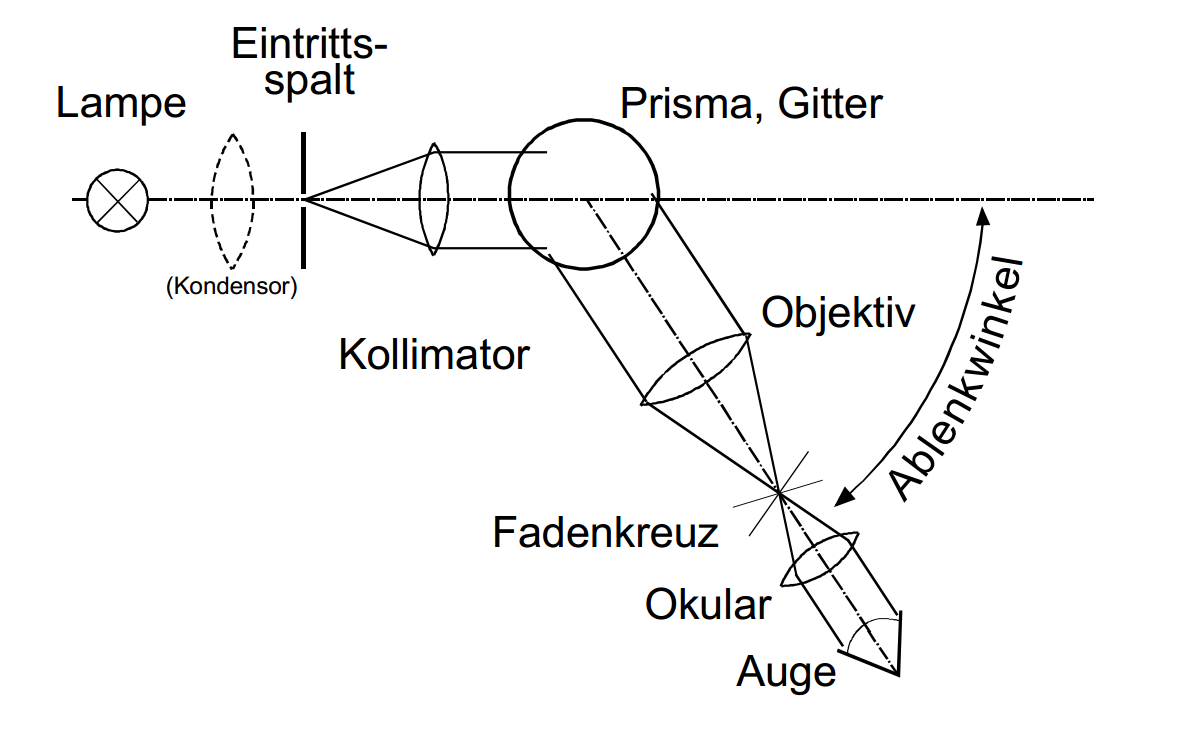
\includegraphics[width=0.8\textwidth]{aufbau.png}
    \caption{Versuchsaufbau}
    \label{fig:aufbau}
\end{figure}

\section{Durchführung}
\subsection{Aufgabe 1}

Nach dem Einschalten der Quecksilberdampflampe haben wir den Aufbau
entsprechend des Skriptes durch Autokollimation justiert. Die Justage war
erfolgreich. Um größtmögliche Messgenauigkeit zu erreichen, haben wir den
Einlassspalt auf den kleinstmöglichen Wert eingestellt.

\subsection{Aufgabe 2}

Entsprechend der Aufgabenstellung wurden die Winkel sowie Farbe und subjektive
Intensität aller sichtbaren Spektrallinien 1. Ordnung aufgenommen. Die Winkel
der Spektrallinien 2. Ordnung wurden nur für die hellsten Linien aufgenommen.
Zur Kontrolle und zur Messung Bestimmung des Winkelnullpunkts wurden diese
Messungen jeweils auf beiden Seiten durchgeführt. Außerdem wurde zur Kontrolle
des Nullpunkts die Linie 0. Ordnung aufgenommen.

\subsection{Aufgabe 3}

Die Lampe wurde gegen eine unbekannte Spektrallampe ausgetauscht. Die Messungen
aus Aufgabe 2 wurden an dieser Spektrallampe wiederholt.

\subsection{Aufgabe 4}

Ein zusätzlicher einstellbarer Spalt wurde hinter dem Kollimator und direkt vor
dem Beugungsgitter eingesetzt. Der Spalt wurde so justiert, dass das
gelb-orange $579{,}1$ / $577{,}0 \operatorname{nm}$ Linienpaar gerade noch im Sinne
des Raygleigh-Kriteriums unterscheidbar war. Die Millimeterschraube des Spaltes
wurde am Nullpunkt und am eingestellten Punkt abgelesen, um aus der Differenz
die Spaltbreite zu ermitteln.

\subsection{Aufgabe 5}

Das Beugungsgitter wurde durch ein Prisma ersetzt und die qualitativen
Beobachtungen notiert.
\newpage
\section{Messwerte}
\newpage
\section{Auswertungen}
\subsection{Aufgabe 1}

Die Justage wurde erfolgreich durchgeführt.

\subsection{Aufgabe 2}
Zur Bestimmung des Nullpunktes haben wir zuerst die 4 prägnantesten Linien
(Violette Hauptlinie, grüne Hauptlinie und gelbe Doppellinie) jeweils ihren
Entsprechungen in den unterschiedlichen Ordnungen anhand von Intensität und
Farbe zugeordnet. Bedeutet konkret: Die violette Hauptlinie der 1. Ordnung
wurde der gegenüberliegenden violetten Hauptlinie der 1. Ordnung zugeordnet,
usw.


% FIXME: Definition Mittelwert, Standardabweichung einbauen.
Durch Berechnung der Mittelwerte der jeweils 2 Werte erhalten wir 8 Nullpunkte.
Durch die Berechnung des Mittelwerts und der Standardabweichung der 8 Werte
erhalten wir den Nullpunkt:

\begin{equation*}
  \alpha_0 = (177{,}98\pm0{,}91)^\circ
\end{equation*}

Dieser ist verträglich mit dem Nullpunkt der durch den Winkel der 0. Ordnung
bestimmt wurde.

Durch Differenzbildung zu diesem Nullpunkt haben wir dann jeweils den
Ablenkwinkel $\alpha$ ermittelt. Da der ermittelte Fehler des Nullpunktes den
Ablesefehler um mehr als eine Größenordnung übersteigt, kann der Ablesefehler
unberücksichtigt bleiben. Der Fehler der Winkel ist somit identisch zum aus der
Streuung ermittelten Fehler.

\begin{equation*}
  \Delta \alpha = 0{,}91^\circ
\end{equation*}

Die ermittelten Werte finden sich in der anliegenden Tabelle.

Die anderen Linien konnten auch durch einen Vergleich mit den Differenzen nicht
eindeutig identifiziert werden, so dass sie für die Ermittlung der
Gitterkonstanten unberücksichtigt bleiben müssen.

Anhand des im Skript enthaltenen Spektrums haben wir den identifizierbaren
Spektrallinien Wellenlängen zugeordnet. Anhand von Gleichung \ref{eq:1} haben
wir dann für jeden Wert eine Gitterkonstante bestimmt.

Anstatt die Gaußßsche Fehlerfortpflanzung zu benutzen, erschien es uns
sinnvoll, da der Fehler des Ablesewinkels ja sowieso durch Streuung bestimmt
wurde, auch den Fehler der Gitterkonstanten aus der Streung zu ermitteln.

Es ergibt sich somit als Zwischenergebnis eine Gitterkonstante von

\begin{equation*}
  d = (1{,}658\pm0{,}055) \operatorname{\mu m}
\end{equation*}

Eine kurze Abschätzung in der Tabellenkalkulation zeigte, dass die Genauigkeit
der Gitterkonstanten nicht ausreichend ist, um auf die Wellenlängen
zurückzurechnen. Die anderen Linien bleiben somit für uns leider nicht
eindeutig identifizierbar.

\subsection{Aufgabe 3}

Nachdem wir die Spektrallinien untereinander zugeordnet haben, haben wir unter
Benutzung der in Aufgabe 2 ermittelten Gitterkonstante die Wellenlänge
bestimmt. Für jede Spektrallinie ergeben sich 4 Wellenlängen. Die tatsächliche
Wellenlänge und den Fehler erhalten wir durch Mittelwertbildung und Berechnung
der Standardabweichung. Gaußsche Fehlerfortplanzung wäre in diesem Fall
möglich, aber da das Ergebnis eindeutig ist, nicht nötig.

Die ersten 3 hellen Spektrallinien lassen sich gut mit den $467{,}8
\operatorname{nm}$, $480{,}0 \operatorname{nm}$ und $508{,}6 \operatorname{nm}$
Linien identifizieren.

Die vierte Linie konnten wir leider in der einen zweiten Ordnung nicht finden,
so dass sich wohl ein systematischer Fehler ergibt, der durch die
Mittelwertbildung nicht aufgehoben wird. Wir können daher nur vermuten, dass es
sich dabei um die hellste Linie handelt, nämlich die $643{,}8
\operatorname{nm}$-Linie.

Da Helium nicht in Frage kommt und die Linien von Zink viel dichter liegen und
daher mit den farblichen Beobachtung nicht übereinstimmen, folgern wir, dass es
sich um eine \textbf{Cadmium-Spektrallampe} handeln muss.

% FIXME: Auswertung
\section{Endergebnis}

\end{document}
